\documentclass[12pt,UTF8,fntef]{article}
\usepackage[left=1.8cm, right=1.8cm, top=1.8cm, bottom=1.8cm]{geometry}
%\usepackage[utf8]{inputenc}
\usepackage[english]{babel}
\usepackage{graphicx}
\usepackage[unicode, pdfborder={0 0 0}, bookmarksdepth=-1]{hyperref}
\usepackage[usenames, dvipsnames]{color}
\usepackage[shortlabels, inline]{enumitem}
\usepackage{fancyhdr}
\usepackage{amssymb}
\usepackage{amsmath}
\usepackage{hyperref}
\usepackage{subfigure}
\usepackage{float}
\usepackage{spreadtab}
\usepackage{booktabs}
%\usepackage{cite}
\usepackage{siunitx}
\usepackage{enumitem}
\usepackage{tikz}
\usepackage{pgfplotstable}

\pgfplotsset{width=15cm}
\pgfplotsset{height=8cm}
\pgfplotsset{compat=1.16}
%\setcitestyle{numbers}

\hypersetup{
    pdftoolbar=true,        % show Acrobat’s toolbar?
    pdfmenubar=true,        % show Acrobat’s menu?
    pdffitwindow=false,     % window fit to page when opened
    pdfstartview={FitH},    % fits the width of the page to the window
    %pdftitle={前瞻語音計畫申請},    % title
    pdfauthor={Jui-Yang Hsu},     % author
    pdfnewwindow=true,      % links in new PDF window
    colorlinks=true,       % false: boxed links; true: colored links
    linkcolor=purple,          % color of internal links (change box color with linkbordercolor)
    citecolor=blue,        % color of links to bibliography
    filecolor=magenta,      % color of file links
    urlcolor=cyan           % color of external links
}

\usepackage[square,numbers]{natbib}
%\bibliographystyle{abbrvnat}
\renewcommand{\baselinestretch}{1.25}
\usepackage{xeCJK}
\usepackage{fontspec}
%\setCJKmainfont{DFFN_R3.TTC}
\setCJKmainfont[BoldFont=Noto Serif CJK TC Bold]{Noto Serif CJK TC}
\title{研究計畫書}
\author{電機工程研究所~~~計算機科學組\\R07921053~~~徐瑞陽 \\ 技術部落格: \texttt{https://sunprinces.github.io/learning/}}
%\email{r07921053@ntu.edu.tw}
\date{}

\begin{document}

\maketitle

近年來深度學習技術已經應用於許多語音的相關領域,並取得突破性的成果,如聲音轉換、智慧問答系統、語音辨識...等,然而這些應用僅限於有豐富標註資料的主流語言。以語音辨識(Automatic Speech Recognition, ASR)為例,利用神經網路與隱式馬可夫模型的混合模型 (DNN-HMM Hybrid Model) 建構以音素 (phoneme) 為單位的聲學模型,再利用發音字典 (lexicon) 與遞歸神經網路 (Recurrent Neural Network) 所訓練的語言模型來做語音辨識為目前最常被使用的架構。然而,這樣的架構除了要有每段語音 (utterance) 對應的翻譯之外,亦需事先用字典及維特比演算法 (Viterbi Algorithm) 對音素及幀 (frame) 做初步對齊後才能進行訓練,因為標註字典的成本昂貴且門檻較高,這樣的設定對於多數非主流研究語言是不切實際的。

因此,Graves 等人提出了端對端語音辨識系統之構想\cite{graves2014towards},近年來也有許多相關模型被提出,如百度的 DeepSpeech \cite{hannun2014deep}、Google 的 LAS \cite{chan2016listen} (架構如 Figure \ref{fig:monoASR} 所示)...等。這些模型主要以序列到序列模型 (Sequence-to-Sequence Model) 作為核心,配合利用專注機制 (Attention) 的解碼器與以 Connectionist Temporal Classification (CTC) 為目標函數的解碼器,訓練出輸入為音訊,輸出為字位 (grapheme) 的端對端模型,同時整合了聲學模型與語言模型的訓練,並移除需要字典的前提。

然而雖然對標註的要求有所降低,相關文獻中均提到了端對端模型相較 DNN-HMM ,若要達到相同詞錯誤率 (Word Error Rate, WER)的情況下,需要更多訓練資料,對於語料量本來就不足的非主流語言來說,這樣的前提也使得該架構難以應用於實務中。也因此,如何利用多語料語言 (high-resource language) 去輔助訓練少語料語言(low-resource language) 的方法 - 語言自適應訓練 (Language Adaptative Training, LAT) 為近年來語音界的主要研究方向之一。接下來,我首先會介紹我所選擇的方法 - 元學習 (Meta Learning),再介紹目前 LAT ASR 的主流方法 - 遷移學習 (Transfer Learning) ,及元學習可能會帶來什麼好處,並展示初步結果及待解決的問題;最後介紹其在生成系列的語音任務如語音合成 (Text-to-Speech, TTS)、聲音轉換 (Voice Conversion, VC)的可能應用。


\newpage

  \begin{section}{元學習介紹}
~~~~目前在監督式學習 (Supervised Learning) - 給定特定任務的大型資料集,從頭開始訓練模型的情境下,深度學習已經取得了很大的成功。然而,相較於人類在學習新任務時,給定少量樣本便能完成學習的情況,其對資料的利用顯然是沒有效率的。而人類之所以能快速學習,主因是我們有元學習 (Meta Learning),又稱為學習如何學習 (Learning to Learn) 的能力,能從先前的任務學習過程中,發現可借鑒的通用經驗,利用已習得的技能,達到快速學習新技能的目的。以下會定義元學習,並介紹及分類近年來提出的方法。

    \begin{subsection}{定義}
      ~~~~以下定義 $\theta$ 為想優化的模型參數,$\mathcal{D}$ 為資料集 ($\mathcal{D}^{\text{tr}}$為訓練資料、$\mathcal{D}^{\text{test}}$為驗證資料),$M$ 為模型 (可以是最近鄰居、類神經網路 $\cdots$),$\mathcal{A}_M(\mathcal{D})$ 為衡量參數在資料集 $\mathcal{D}$ 上好度的函數, 我們想找到一個模型 $f_\theta: \mathcal{D} \rightarrow M$ 滿足以下元學習的目標。
      \begin{equation}
        \theta^{\star} = \arg \max_\theta \mathbb{E}_{\mathcal{D} \sim p(\mathcal{D}) }[\mathcal{A}_{f_\theta(\mathcal{D^{\text{tr}}})}(\mathcal{D^{\text{test}}})]
      \end{equation}

而不同 $f_\theta$ 的實現方式,也對應了不同的元學習算法,以下介紹目前主流的三種方法。



      %為了更好的理解元學習,我們來看一個其最常被使用的情境 - 少量樣本分類 (Few-shot Classification)。在這樣的情境下,對每個任務 (task) 我們都只有少量的訓練資料,但有多個任務可以學習。舉例來說,我們擁有數個二元分類的資料集 (狗 vs 貓, 火車 vs 飛機, 蘋果 vs 香蕉...),但每個資料集的每個類別都只有 $N$ 個訓練樣本 ($N \geq 1$),給定一個新資料集 (鳥 vs 船,且此類別都沒有出現在先前的資料集中),我們希望訓練出的模型能做到僅利用 $2N$ 張樣本便自適應 (adapt) 到新資料集上。

      %在這樣的情境下,對於每個特定任務我們都只有少量的訓練資料,但有多個任務可以學習,目標為

      %\begin{equation}
   %\theta^\star = \arg \max_\theta \mathbb{E}_{L \subset \mathcal{L}} \, [ \mathbb{E}_{S^L \subset \mathcal{D}, B^L \subset \mathcal{D}}[\sum_{(x,y) \in B^L} \log P_\theta(y|x,S^L)] \,  ]
       %\end{equation}
    \end{subsection}

    \begin{subsection}{基於度量的元學習方法 (Metric-based Approach)}
      $f_\theta$的主體在學習一個特徵編碼器 (feature encoder),而經過該編碼器編碼後的特徵,再用最近鄰居 (Nearest Neighbor) 算法解決分類問題。如原型網路 (Prototypical Network) \cite{snell2017prototypical}、配對網路 (Matching Network)\cite{vinyals2016matching}...等, 此方法目前僅用於分類。
    \end{subsection}

    \begin{subsection}{基於模型設計的元學習方法 (Model-based Approach)} \label{model-meta}
      $f_\theta$的主體為一個複雜的模型 (神經網路及其變形),藉由設計該模型架構,使得輸入資料集後能吐出 $M$的參數,或再接著輸入測試樣本的資料點後直接輸出預測。舉例來說,記憶增強網路 (Memory Augmented Network) \cite{santoro2016meta}利用神經圖靈機,建構一個可讀寫的外部記憶,用來儲存訓練樣本以便預測時查找。
    \end{subsection}

    \begin{subsection}{基於梯度優化的元學習方法 (Gradient-based Approach)} \label{opt-meta}
      $f_\theta$的主體為將 $\theta$ 嵌至模型的超參數之中 (如起始參數、模型架構 $\cdots$),之後利用訓練資料做幾步的梯度下降 (Gradient Descent) 後用來在測試資料的預測,當中嵌入起始參數的方法 \cite{finn2017model, nichol2018first},也可看成是一種預訓練 (Pretraining) 的方式。需注意的是,利用這組參數直接在新資料集上進行預測並不能得到理想的結果,而是需要先進行幾步的梯度下降更新。
    \end{subsection}
  \end{section}
  \newpage


  \begin{section}{元學習應用於語言自適應訓練 (LAT)}
    \begin{subsection}{過去主流的語言自適應訓練方法 - 遷移學習} \label{trans-asr}

    \begin{figure}[ht]
        \centering
        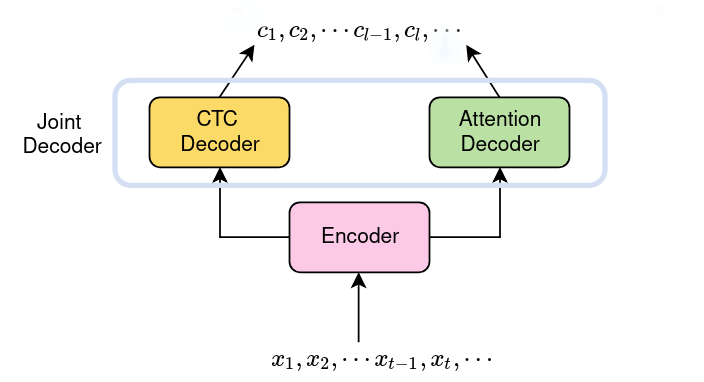
\includegraphics[width=0.6\linewidth]{monoASR.png}
        \caption{Basic learner structure: LAS}
        \label{fig:monoASR}
    \end{figure}

    \vspace{-0.25in}

    \begin{figure}[ht]
      \centering
      \subfigure[Universal ASR: Union the output classes]{%
        \label{fig:universalASR}%
      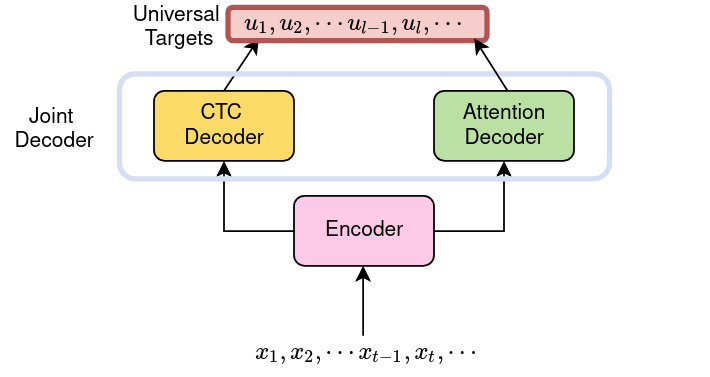
\includegraphics[width=0.55\linewidth]{UniversalASR.png}}%
      \subfigure[MultiTask ASR: Language-specific decoder]{%
        \label{fig:multitaskASR}%
      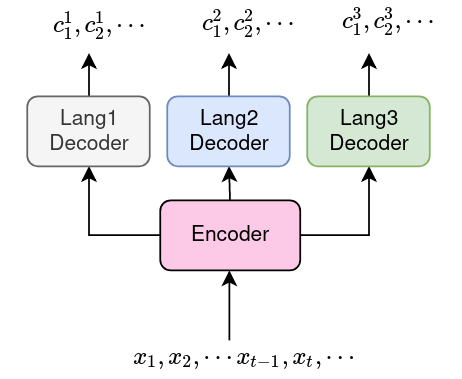
\includegraphics[width=0.41\linewidth]{MultiTaskASR.png}}%
      \caption{Baseline model: Universal ASR \& MultiTask ASR}
    \end{figure}

    目前端對端語音辨識模型 LAT 的主流方法為遷移學習。其中 Figure \ref{fig:monoASR} 為基本的模型架構,可以訓練單一語言的模型。Figure \ref{fig:universalASR} 則延伸原先的架構,統一所有訓練語料的輸出類別,可藉由聯集訓練語言的字位或使用語言通用的國際音標來實現;Figure \ref{fig:multitaskASR} 架構則是對不同語言建構各自的解碼器,分別輸出字位,但前面的編碼器是互相共享的。在遷移到目標語言時,我們將輸出層換成適合該語言的層,並重新訓練輸出層,或對整個模型進行微調 (fine-tuning) 以實現 LAT\footnote{此處不考慮將目標語言加入訓練,雖然這通常會讓結果更好,但我們希望訓練的模型對目標語言沒有任何假設}。

  ~~在編碼器端,為了消弭不同語言的差異,擷取出語言獨立 (language-independent) 的特徵供解碼器使用,常見的作法有加上語言分類器進行對抗訓練 (Adversarial Training),或加入音素、子字單位 (subword unit)的 CTC 解碼器。
    \end{subsection}


    \begin{subsection}{為何元學習於語音有研究價值}

  \begin{figure}[ht]
      \centering
      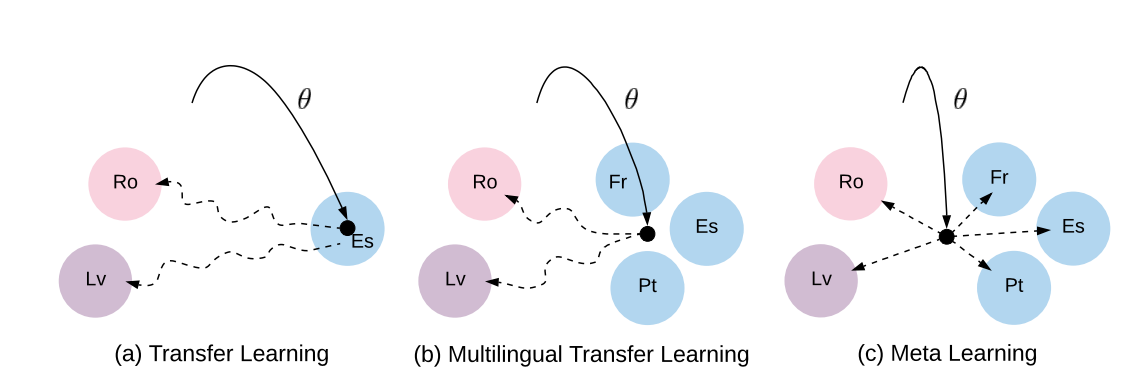
\includegraphics[width=0.8\linewidth]{Meta-motivation.png}
      \caption{不同學習之間的比較,實線為初始參數的學習過程,虛線為微調的過程}
      \label{fig:motivation}
  \end{figure}

  遷移學習以一個在多語料(多語言)訓練好的模型為基準,用於學習新的目標語言,如Figure \ref{fig:motivation} 的 (a)、(b)\footnote{圖片來自 \cite{gu2018meta}},然而問題有二︰
      \begin{enumerate}[itemsep=-1mm]
        \item 需假設訓練語料彼此的最優參數不能相差太多,因在訓練過程中必須同時滿足各語言的目標函數,這相當於對模型施加了正則化 (regularization),使其無法很好處理語種差異過大,導致正則化強度太大,無法達到最佳表現的情況。
        \item 需假設訓練語料與測試語料的最優參數不能相差太多,否則在損失平面 (loss surface) 上過長的移動,會降低找到好解的可能。 
      \end{enumerate}

      元學習中基於梯度優化的方法(\ref{opt-meta}) 實驗上緩解了上述問題,透由在梯度更新時,將學習過程隱性編碼進所找到的參數中,使得該參數可以快速泛化到不同語言,如 Figure \ref{fig:motivation} 的 (c) 所示。
    \end{subsection}
    %\begin{subsection}{使用限制及挑戰} \label{meta-problem}
      %目前元學習主要應用於機器視覺的少樣本分類、與強化學習,直至去年,才有了第一篇應用於機器翻譯的研究 \cite{gu2018meta},MetaNMT,訓練多語言翻譯至英文的模型,原因為以下兩點︰
      %\begin{enumerate}[itemsep=-1mm]
        %\item 要訓練一個成功的機器翻譯或語音辨識系統,難度相當高,不可能僅僅使用數個樣本便達到,因此多數針對少樣本分類問題的元學習演算法不適用,僅有基於優化的演算法 (\ref{opt-meta}) 在以一階梯度近似的前提下才能應用於該情境 (如 FOMAML \cite{finn2017model}、Reptile\cite{nichol2018first})。
        %\item 多數學習初始參數的元學習方法雖名為與模型無關 (Model-Agnostic) ,但在使用時仍要求模型架構必須相同 (如網路中每層的神經元數量),MetaNMT 的處理方式為先將所有語言映射到相同空間,使得輸入層一致進而達到全模型一致;但在語音辨識中,雖然不同語言的輸入同為相同維度的語音特徵,輸出卻是每個語言都不同,因此無法直接套用元學習。
      %\end{enumerate}
    %\end{subsection}
    \begin{subsection}{實驗 - 端對端語音辨識} \label{progress}
      在端對端的語音辨識中,我選用 IARPA-BABEL 這個語料庫做為評斷標準,該語料庫包含了 $10$ 餘種語言,每個語言約有 $40 \sim 80$ 小時不等的語料,當中又分為兩個資料集,FLP (Full Language Pack) 為所有的訓練語料,而 LLP (Limited Language Pack) 則是根據 Kaldi 處方從 FLP 中所選出的約 $10$ 小時的語料。我採用不同語言的 FLP ,包含 Bengali (Bn), Tagalog (Tl), Zulu (Zu), Turkish (Tr), Lithuanian (Lt), Telugu (Te) 之組合作為預訓練語料,來測試在另外四種語言上的遷移成效,包含了 Vietnamese (Vi), Swahili (Sw), Tamil (Ta), Kurmanji (Ku),所採用的模型架構為 Figure \ref{fig:multitaskASR}\footnote{Figure \ref{fig:universalASR} 的架構的遷移成效不佳,故在此不回報},底下所提到的 MultiASR 為從所有預訓練文本中隨機抽取資料,訓練共享的特徵編碼器,及對應的語言輸出層,而 MetaASR 則是採用 Finn et al. 所提出的 Model Agnostic Meta Learning (MAML, \cite{finn2017model}) ,將不同語言視為不同任務,並仿照其更新步驟而得。
    \end{subsection}

    \begin{subsection}{初步結果}
      \begin{table*}[thp!]
\centering
\caption{字錯誤率 (Character error rate, \si{\percent} CER) 於欲遷移語言的 FLP 的測試集}
\label{tab:flp-table}
\begin{tabular}{@{}ccccccccc@{}}
%\begin{tabular}{l|cc|cc|cc|cc}
\toprule
Model                                    & \multicolumn{2}{c}{Vietnamese}                         & \multicolumn{2}{c}{Swahili}                        & \multicolumn{2}{c}{Tamil}                        & \multicolumn{2}{c}{Kurmanji} \\

                                         & multi           & meta                                & multi           & meta                                & multi           & meta                                & multi           & meta           \\ \midrule
\multicolumn{1}{c|}{(no-pretrain)}                   & \multicolumn{2}{c|}{56.5}                    & \multicolumn{2}{c|}{45.3}                    & \multicolumn{2}{c|}{69.9}          & \multicolumn{2}{c}{61.1}                    \\

\multicolumn{1}{l|}{Bn Tl Zu}   &    60.9      & \multicolumn{1}{c|}{49.6}          & 48.1          & \multicolumn{1}{c|}{38.3}          & 65.6          & \multicolumn{1}{c|}{57.5}          & 61.6          & 58.8          \\
\multicolumn{1}{l|}{ \qquad \qquad Tr Lt Gn} & 53.3          & \multicolumn{1}{c|}{49.9}          & 44.3          & \multicolumn{1}{c|}{39.3}          & 68.2          & \multicolumn{1}{c|}{57.7}          & 58.8          & 59.9          \\
\multicolumn{1}{l|}{Bn Tl Zu Tr Lt Gn}           & 65.6          & \multicolumn{1}{c|}{50.1}          & 48.4          & \multicolumn{1}{c|}{38.8}          & 65.6          & \multicolumn{1}{c|}{58.9}          & 62.2          & 57.6          \\ \bottomrule
\end{tabular}
\end{table*}

從上表可以看出,遷移學習帶來了一定的成效,而以 MetaASR 作為預訓練的模型,相較 MultiASR 在遷移上的成效是更為顯著的。我們同時也展示了不同預訓練步數 (Pretraining Step) 對遷移語言之驗證集的詞錯誤率之關係圖,如 Figure \ref{fig:learning-curve} 所示,可以看出隨著預訓練步數的增加,MetaASR 的遷移成效並不似 MultiASR 下降,這裡因空間限制,僅選用了一組預訓練語言與欲遷移語言的組合作為展示,但我們在所有的組合上均觀察到此現象。

\begin{figure}[ht]
  \centering
  %\hspace{-2.2cm}
  \begin{tikzpicture}
  %\begin{tikzpicture}[trim axis left, trim axis right]

  \begin{axis}[
    width=\linewidth,
    height=6.0cm,
    %legend entries={MultiASR, MetaASR} ,
    legend entries={MultiASR, MetaASR, no-pretrain} ,
    xlabel = {Number of pretraining steps ($\times 1000$)},
        xmin=5,
        %xmax=130,
        grid=both,
        legend style={at={(0.02,0.48)},anchor=south west},
        %legend pos=inner north west,
        ylabel={CER (\si{\percent}})]
  \addplot+[smooth]table{multi6-swahili};
  \addplot+[smooth]table{meta6-swahili};
   \addplot[style=ultra thick,dashed,] coordinates {(0,64.3) (100,64.3)};
  \end{axis}
  \end{tikzpicture}
  \center \caption{Learning curves on Swahili's LLP (pretrained on Bn, Tl, Zu, Tr, Lt, Gn)}
  \label{fig:learning-curve}
\end{figure}
    \end{subsection}

    \begin{subsection}{未來發展}
      從 Table \ref{tab:flp-table} 可以看出,即使增加預訓練語言的種類,對遷移成效的幫助有限,這與我們預期的結果並不相符,我想以 MAML 作為基礎,發展新的方法去增進其在遷移上的效率,並測試在更多種類的語料上,如 \cite{black2019cmu} \footnote{他們團隊抓取語料的腳本之連結,從去年 3 月壞掉現在尚未更新}或預訓練語種與遷移語言的組合。要達成以上目標,我們需要檢驗以下
      \begin{enumerate}
        \item 切除研究 (Ablation Study) 來觀察元學習帶來進步的表現可能是來自更有效率地學習語言模型/聲學模型。
        \item 測試在不同的模型架構上,如 DeepSpeech, Wav2letter,觀察遷移成效是否與模型無關 (model-agnostic)。
        \item 觀察何處可能是造成負遷移 (Negative Transfer) 的原因,在目標函數或原有的演算法中加入限制去減緩。
        %\item 要訓練一個語音辨識系統,難度相當高,很難僅僅用數個樣本便達到,因此多數針對少樣本分類問題的元學習演算法不適用,僅有基於優化的演算法 (\ref{opt-meta}) 在以一階梯度近似的前提下才能應用於該情境 (如 FOMAML \cite{finn2017model}、Reptile\cite{nichol2018first})。
      \end{enumerate}
    \end{subsection}
\end{section}

\begin{section}{元學習於生成系語音任務}
  目前元學習中僅有極少數用於語音生成任務的研究(\cite{chen2018sample, serra2019blow}) ,均為利用基於模型的元學習方法 (\ref{model-meta}),尚無基於梯度優化的方法(\ref{opt-meta})。因此將 \ref{opt-meta} 的方法套用在生成模型上,如變分自特徵編碼器 (Variational AutoEncoder, VAE)、生成對抗式網路 (Generative Adversarial Network, GAN) $\cdots$ 等,並利用元學習能用少量樣本達成任務的特性,將想分開來估測的資料視為不同任務(如不同語者的特性、背景音 $\cdots$),在 TTS, VC 的任務上生出更高品質的語音,亦為有相當潛力的方向。
\end{section}



\bibliographystyle{plainnat}
\bibliography{M335}

\end{document}
